\tikzstyle{pic}=[inner sep=0pt]
\tikzstyle{quote}=[fill=gray!30, inner sep=12pt]

\newcommand{\vogels}{
  \node[pic] (vogels) at (0, 0) {
    
\includegraphics[
      width=0.22\textwidth,
      trim=0 75 0 25,
      clip
    ]{assets/vogels.jpg}
  };
}

\newcommand{\hoare}{
  \node[pic, right=0.2cm of vogels] (hoare) {
    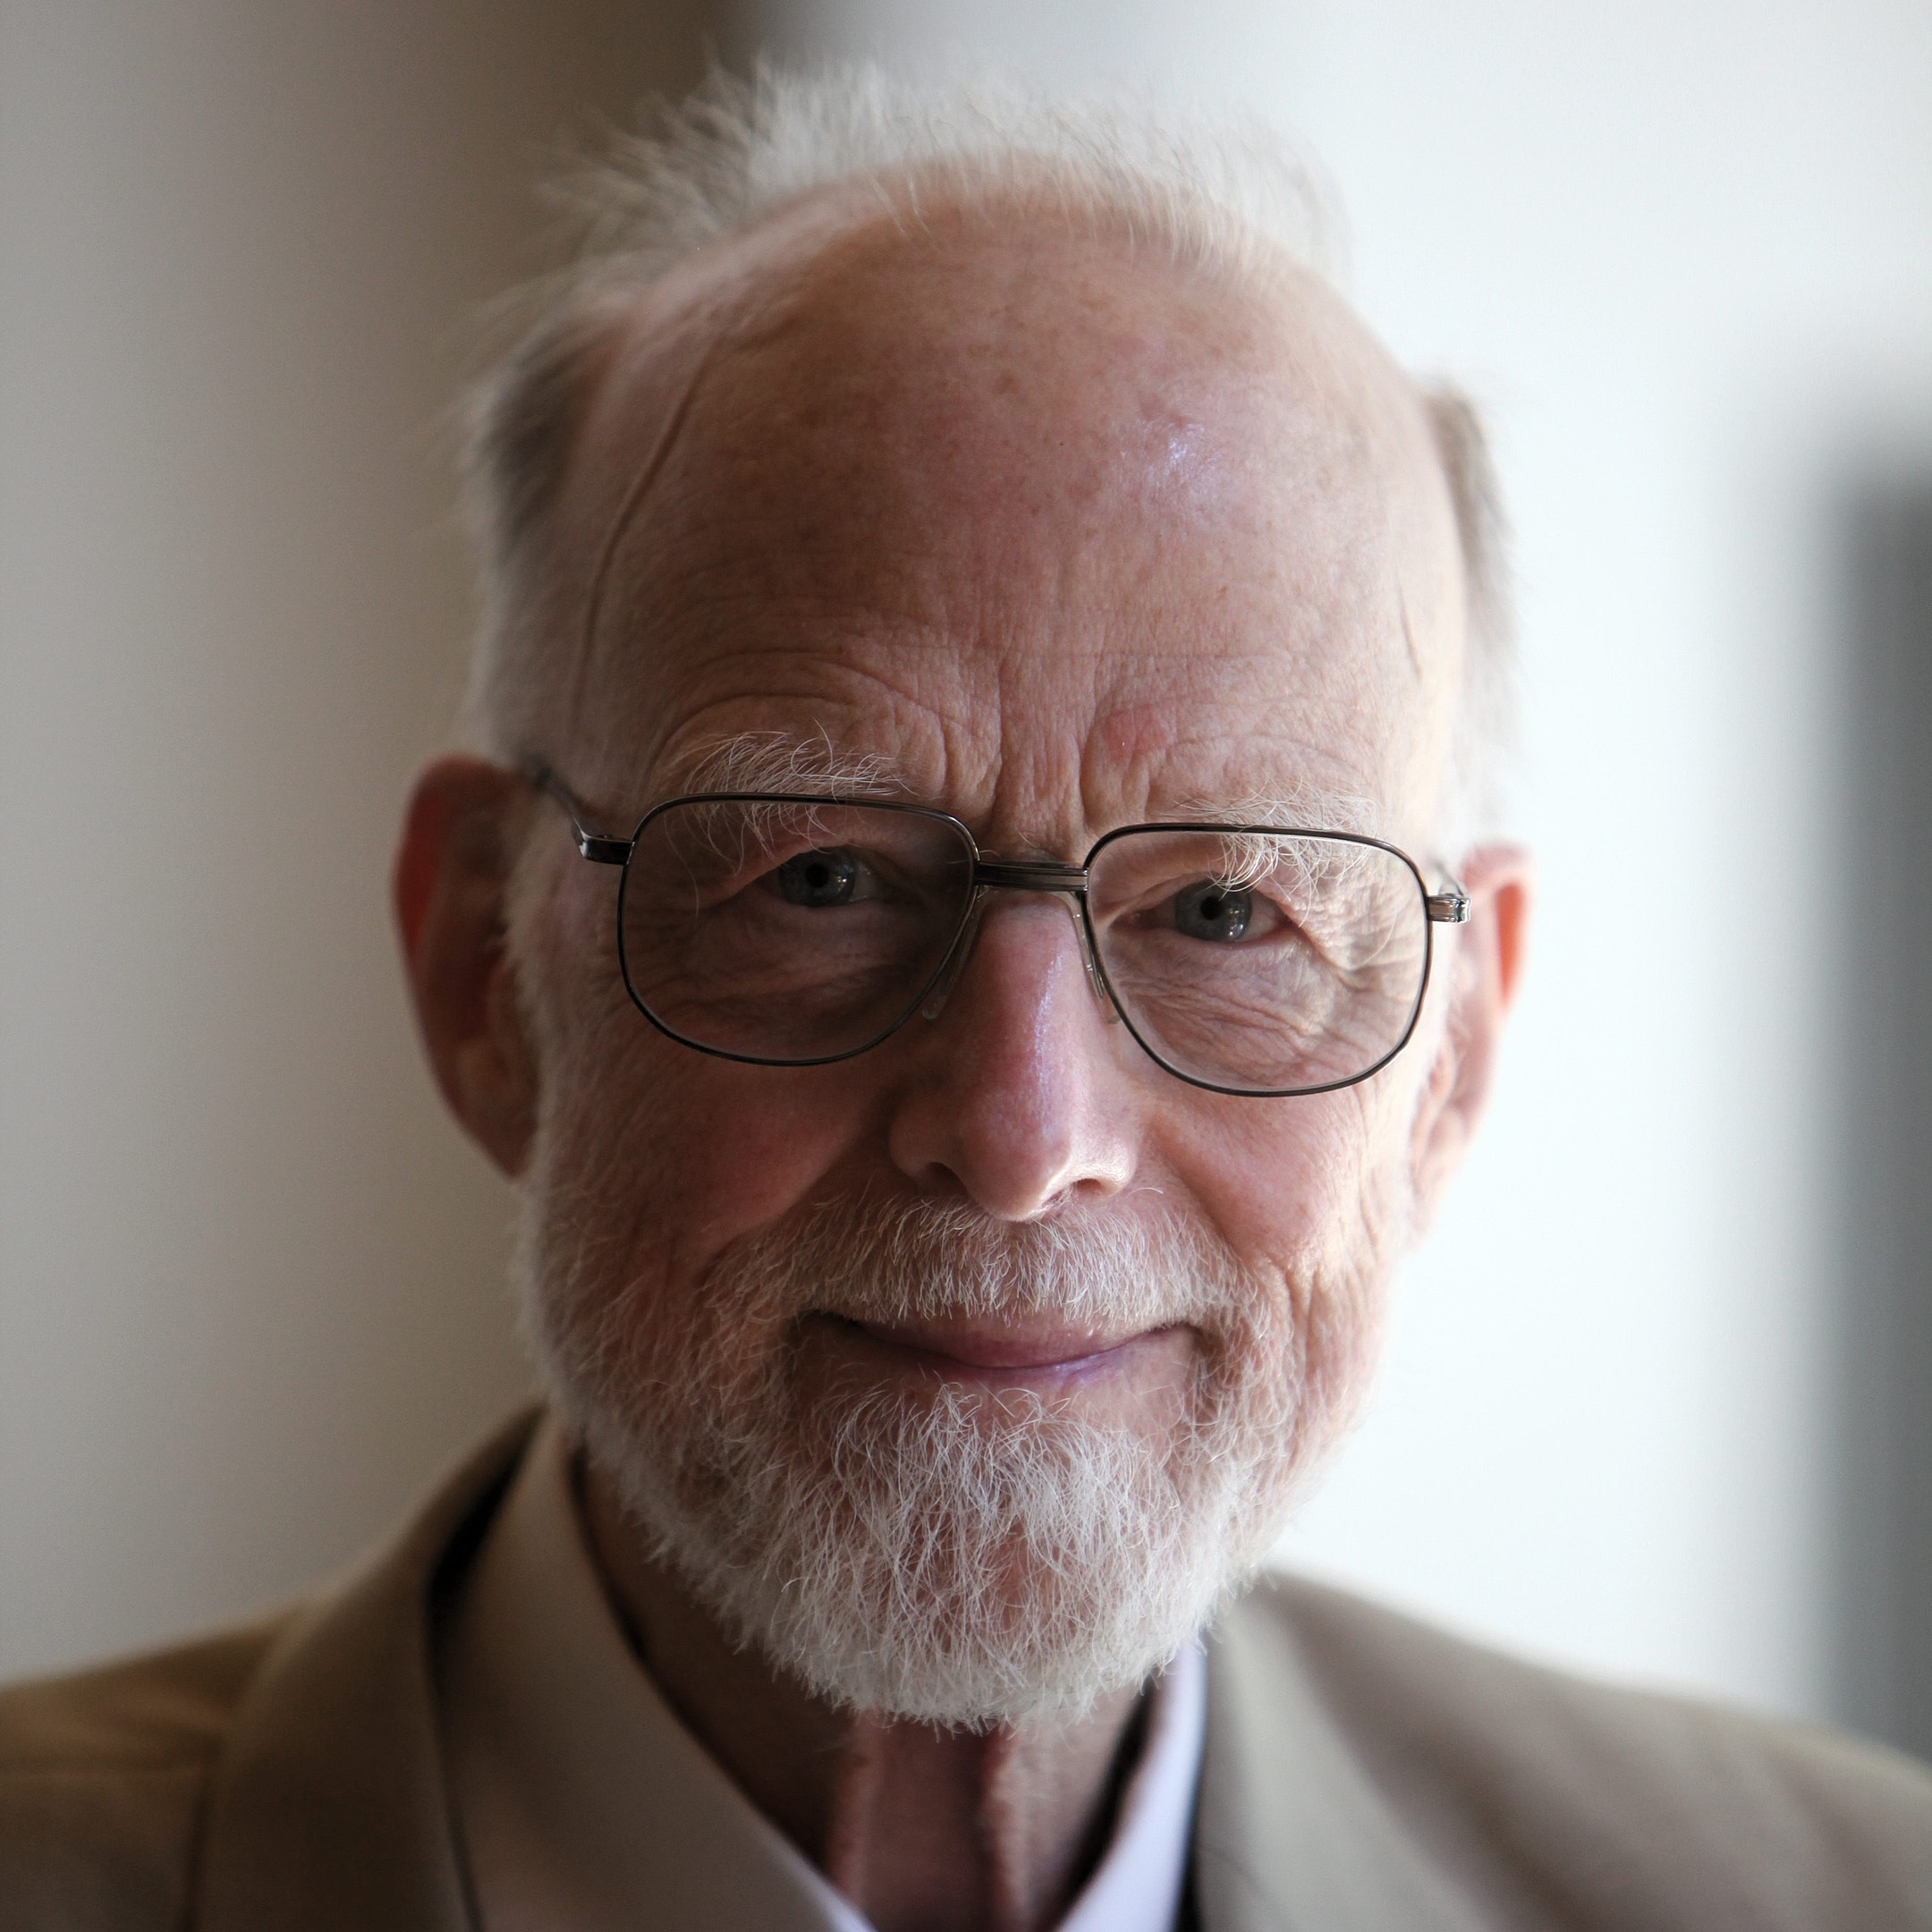
\includegraphics[width=0.22\textwidth]{assets/hoare.jpg}
  };
}

\newcommand{\lamport}{
  \node[pic, right=0.2cm of hoare] (lamport) {
    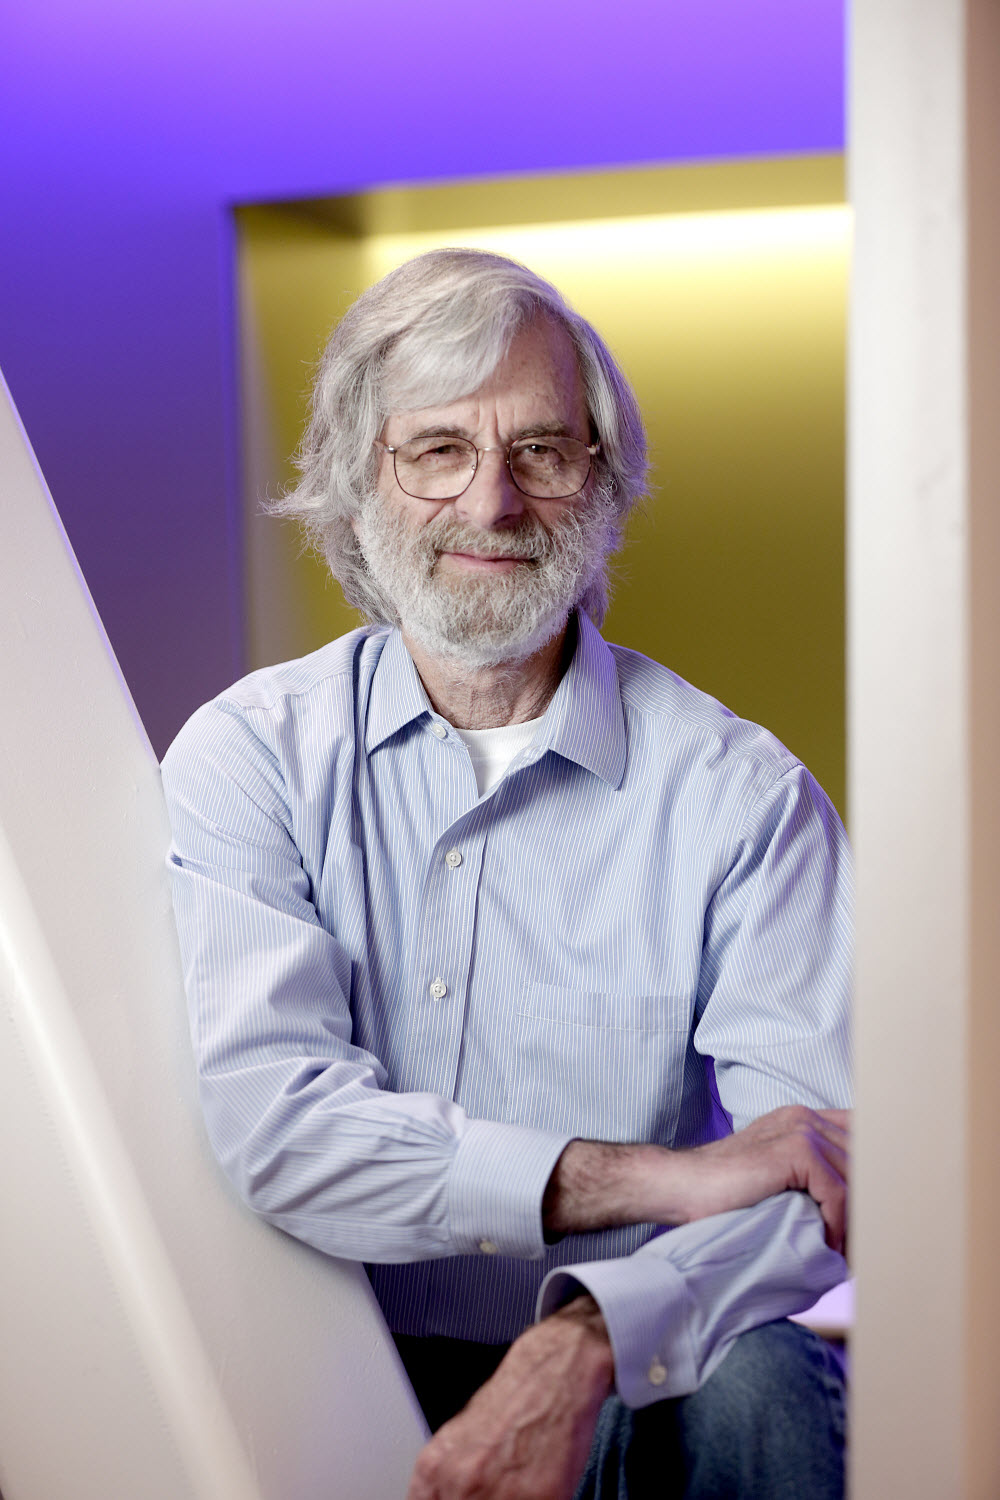
\includegraphics[
      width=0.22\textwidth,
      trim=250 700 300 200,
      clip
    ]{assets/lamport.jpg}
  };
}

\newcommand{\brewer}{
  \node[pic, right=0.2cm of lamport] (brewer) {
    
\includegraphics[
      width=0.22\textwidth,
      trim=100 300 100 100,
      clip
    ]{assets/brewer.jpg}
  };
}

\begin{frame}
  \note{%
    Hi everyone! Thanks so much for attending. I'm Michael, and today I'll be
    talking about ``Interactive Checks for Coordination Avoidance''. This is
    joint work with my advisor at UC Berkeley, Joe Hellerstein.

    Imagine you're an application developer and you're trying to decide what
    kind of consistency you'd like to use to replicate some of your data.
  }
\end{frame}

\begin{frame}
  \begin{center}
    \begin{tikzpicture}[xscale=1.3]
      \vogels
      \node[quote, text width=0.8\textwidth, align=left] at (0, 3) {
        \Large\textit{You should use weak consistency. It's wicked fast!}
      };
      \path[fill=gray!30] (vogels.north) -- ++(0, 1) -- ++(0.5, 0) -- (vogels.north);
    \end{tikzpicture}
  \end{center}

  \note{%
    Someone like Werner Vogels would probably tell you to use weak consistency.
    You can implement weak consistency super duper fast, and for many
    applications, weak consistency is good enough.
  }
\end{frame}

\begin{frame}
  \begin{center}
    \begin{tikzpicture}[xscale=1.3]
      \vogels
      \hoare
      \node[quote, text width=0.8\textwidth, align=left] at (1, 3) {
        \Large\textit{What about the application invariants?!}
      };
      \path[fill=gray!30] (hoare.north) -- ++(0, 1.5) -- ++(1, 0) -- (hoare.north);
    \end{tikzpicture}
  \end{center}

  \note{%
    But then Tony Hoare laments, ``no no no''. Hoare encourages us not to
    settle for weak consistency because a weakly consistent system is hard to
    reason about. It robs us of a fundamental way we use to reason about
    programs: application invariants. Even if every transaction in a weakly
    consistent system preserves application invariants, the whole system may
    not.
  }
\end{frame}

\begin{frame}
  \begin{center}
    \begin{tikzpicture}[xscale=1.3]
      \vogels
      \hoare
      \lamport
      \node[quote, text width=0.8\textwidth, align=left] at (2, 3) {
        \Large\textit{Yeah, go with strong consistency! I have an algorithm for that :)}
      };
      \path[fill=gray!30] (lamport.north) -- ++(0, 1.5) -- ++(1, 0) -- (lamport.north);
    \end{tikzpicture}
  \end{center}

  \note{%
    Leslie Lamport chimes in agreeingly. He encourages us to choose strong
    consistency. Strongly consistent systems are much easier to reason about.
    After all a strongly consistent system to end users looks exactly like a
    system that's not even distributed.
  }
\end{frame}

\begin{frame}
  \begin{center}
    \begin{tikzpicture}[xscale=1.3]
      \vogels
      \hoare
      \lamport
      \brewer
      \node[quote, text width=0.8\textwidth, align=left] at (3, 3) {
        \Large\textit{Not so fast!}
      };
      \path[fill=gray!30] (brewer.north) -- ++(0, 1.5) -- ++(-1, 0) -- (brewer.north);
    \end{tikzpicture}
  \end{center}

  \note{%
    ``Aha, not so fast'' counters Eric Brewer! Consistency and availability and
    partition tolerance, oh my. Surely, strong consistency comes at the price
    of availability and performance.

    So we're in a bit of a pickle. Weak consistency is too confusing and strong
    consistency is too heavy handed.
  }
\end{frame}

\begin{frame}
  \begin{center}
    \begin{tikzpicture}[xscale=1.3]
      \node[pic] (bailis) at (0, 0) {
\includegraphics[width=0.25\textwidth]{assets/bailis.jpg}};
      \node[quote, text width=0.8\textwidth, align=left] at (0, 3) {
        \Large\textit{?`Porque no los dos?}
      };
      \path[fill=gray!30] (bailis.north) -- ++(0, 1.5) -- ++(1, 0) -- (bailis.north);
    \end{tikzpicture}
  \end{center}

  \note{%
    Thankfully, Peter Bailis comes to save the day and reminds us that perhaps
    we can have the best of both worlds. In 2014, Peter and some other smart
    folks defined invariant confluence as a condition under which we can
    replicate a piece of data without the need for strongly consistent
    coordination while maintaining the data's application invariants.

    Invariant confluence will be the topic of this talk. In particular, I'll
    define invariant confluence and then discuss how we can check invariant
    confluence automatically.
  }
\end{frame}
